TRITIUM-IFIC-0 was the first prototype developed in the TRITIUM project aiming to prove the feasibility of the technology proposed by TRITIUM, that is, to employ plastic scintillating fibres to detect tritium in water with sufficient sensitivity. As liquid radioactive sources were involved, special attention was paid to radiation safety in the design.

TRITIUM-IFIC-0 consists of a bundle of 35 fibres $20~\cm$ long, which were cleaved and polished with the techniques reported in section \ref{sec:CharacterizationScintillatingFibers}. This bundle is attached to the vessel through metallic pieces located at its ends, as shown in Figure \ref{fig:FiberBundleOfTritiumIFIC0}. The PVC\footnote{Polyvinyl Chloride, PVC} vessel, shown in Figure \ref{fig:TritiumIFIC0}, was designed in a U-shape to improve radiological safety. However, this shape was not appropriate as we learned afterwards. A frame of methacrylate and steel, shown in Figure \ref{fig:TritiumIFIC0}, was designed and built to hold the prototype. Two calibrated Hamamatsu R8520-06SEL PMTs \cite{DataSheetPMTs} were coupled to the fibre bundle with optical grease \cite{OpticalGrease}. The voltage divider circuit employed is shown in Figure  \ref{fig:VoltageDividerCircuit}. The high voltage was set to $-800~\volt$, at which the gains are $1.26 \cdot{} 10^6$ and $1.01 \cdot{} 10^6$, and the quantum efficiencies are $29.76\%$ and $28.66\%$ at $\lambda=430~\nano\meter$, respectively. The two PMTs were read out in coincidence by the electronics shown in Figure \ref{subfig:ElectronicConfiguraiton2PMT}.

\begin{figure}
\centering
    \begin{subfigure}[b]{0.5\textwidth}
    \centering
    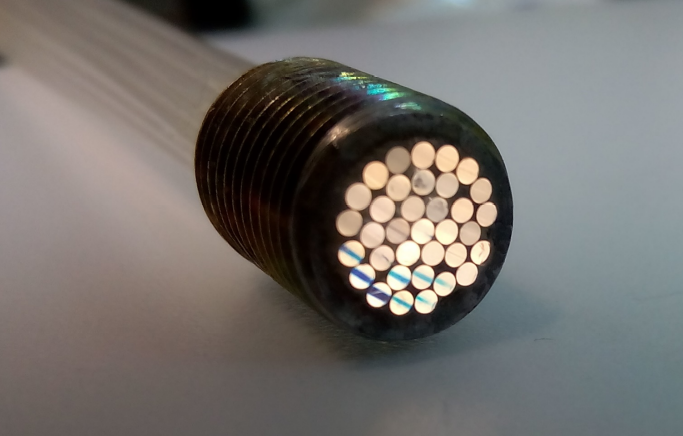
\includegraphics[width=\textwidth]{5Prototypes/52PreliminarPrototypes/521TritiumIFIC0/Metalic_piece_of_fiber_bundle.png}  
    \caption{\label{subfig:MetalicPieceFiberBunchTritiumIFIC0}}
    \end{subfigure}
    \hfill
    \begin{subfigure}[b]{0.4\textwidth}
    \centering
    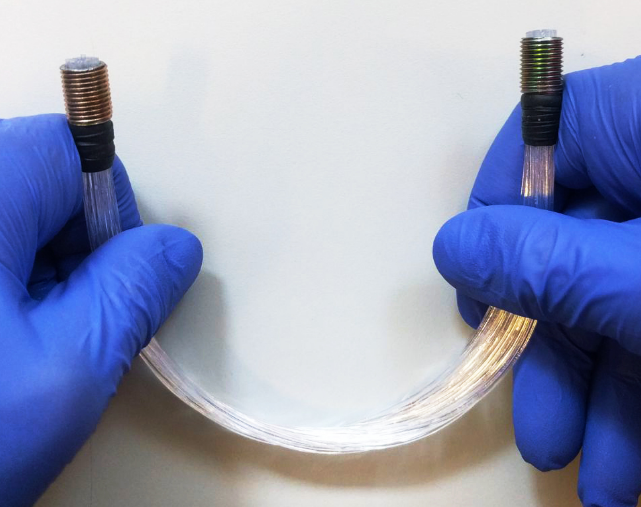
\includegraphics[width=\textwidth]{5Prototypes/52PreliminarPrototypes/521TritiumIFIC0/FiberBundleBent.png}  
    \caption{\label{subfig:FiberBunchTritiumIFIC0Bent}}
    \end{subfigure}
 \caption{a) Metallic piece of the fibre bundle. b) Bundle of $35$ fibres of $20~\cm$ length used in TRITIUM-IFIC-0.} \label{fig:FiberBundleOfTritiumIFIC0}
\end{figure}

\begin{figure}[h]
\centering
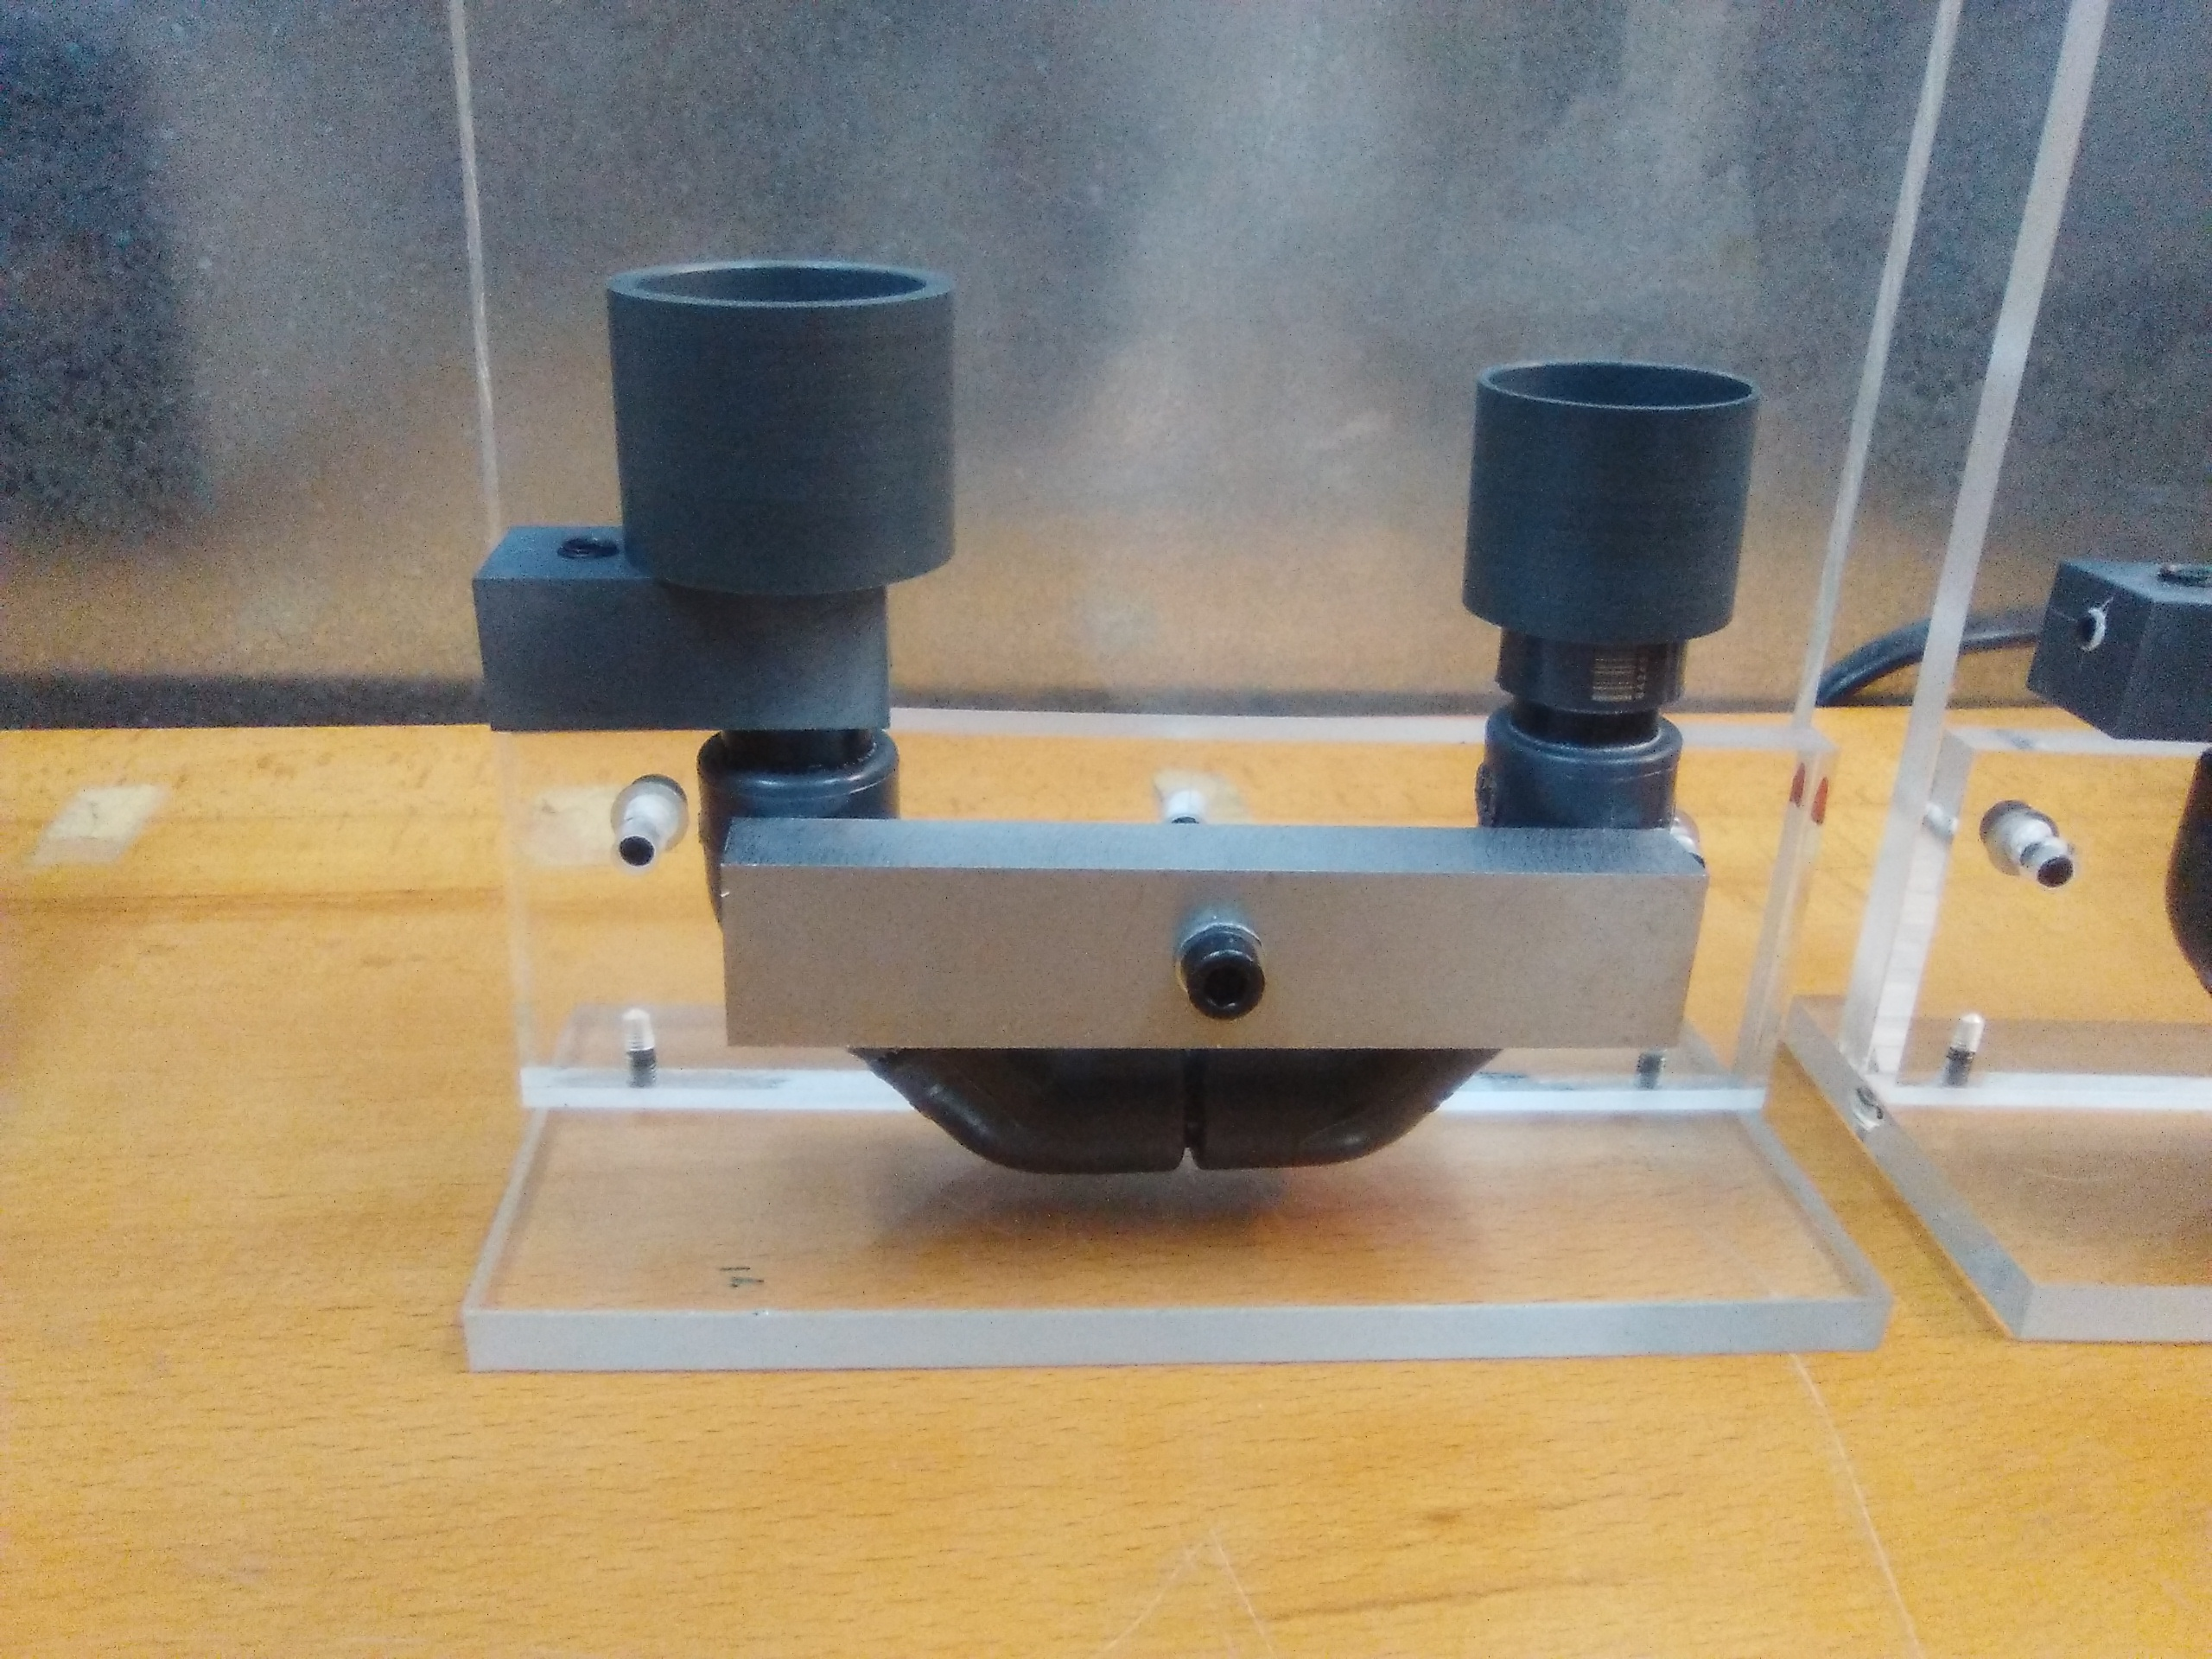
\includegraphics[scale=0.12]{5Prototypes/52PreliminarPrototypes/521TritiumIFIC0/Tritium_IFIC_0.jpg}
\caption{TRITIUM-IFIC-0 prototype.\label{fig:TritiumIFIC0}}
\end{figure}

Two identical prototypes were built. The first one, called ``TRITIUM-IFIC-0 Background'', was filled with pure water ($39~\milli\liter$, uncertainty of $0.05\%$) and was used to measure the background, whereas the second one, called ``TRITIUM-IFIC-0 Signal'', was filled with a radioactive liquid source of tritiated water of specific activity of $99.696~\kilo\becquerel/\liter$ ($2.24\%$ uncertainty) as reported in Appendix \ref{App:TritiumSourcePreparation}. This second prototype was employed to measure the total signal (tritium + background). The tritium signal was determined by subtracting the background from the total signal. The number of coincident events was too low due to photon escape from the fibers caused by several reasons such as the excessive curvature of the fibre bundle and the poor quality of the interface between tritiated water and fibres. The implementation of the cleaning process described in section \ref{sec:CharacterizationScintillatingFibers} was motivated by this result. 

A transparent glass vessel similar to the TRITIUM-IFIC-0 prototype vessel, shown in Figure \ref{subfig:PMMAVesselToTestLostPhotons}, was built to study the effect of the fibre bundle curvature. The LED described in section \ref{sec:CharacterizationScintillatingFibers} was used to asses the reduction in photon collection of the fibre bundle. As can be seen in Figure \ref{subfig:TestLostPhotons}, most of the photons introduced from one side of the bundle do not reach the other side. This test showed essential to keep a straight fibre arrangement in the design of the next prototypes. A second point is that the fibre bundle was too compact which possibly prevented water from flowing adequately between the fibres. In the TRITIUM-IFIC-1, the fibres were sufficiently spaced by using a PTFE matrix.

\begin{figure}
\centering
    \begin{subfigure}[b]{0.45\textwidth}
    \centering
    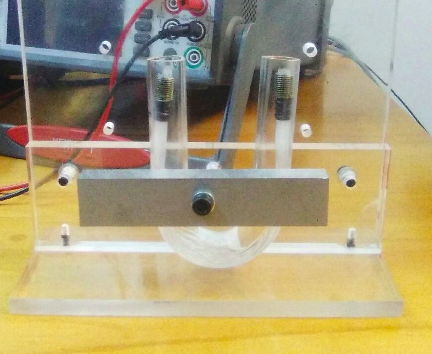
\includegraphics[width=\textwidth]{5Prototypes/52PreliminarPrototypes/521TritiumIFIC0/PMMA_vessel_ZOOM.png}  
    \caption{\label{subfig:PMMAVesselToTestLostPhotons}}
    \end{subfigure}
    \hfill
    \begin{subfigure}[b]{0.45\textwidth}
    \centering
    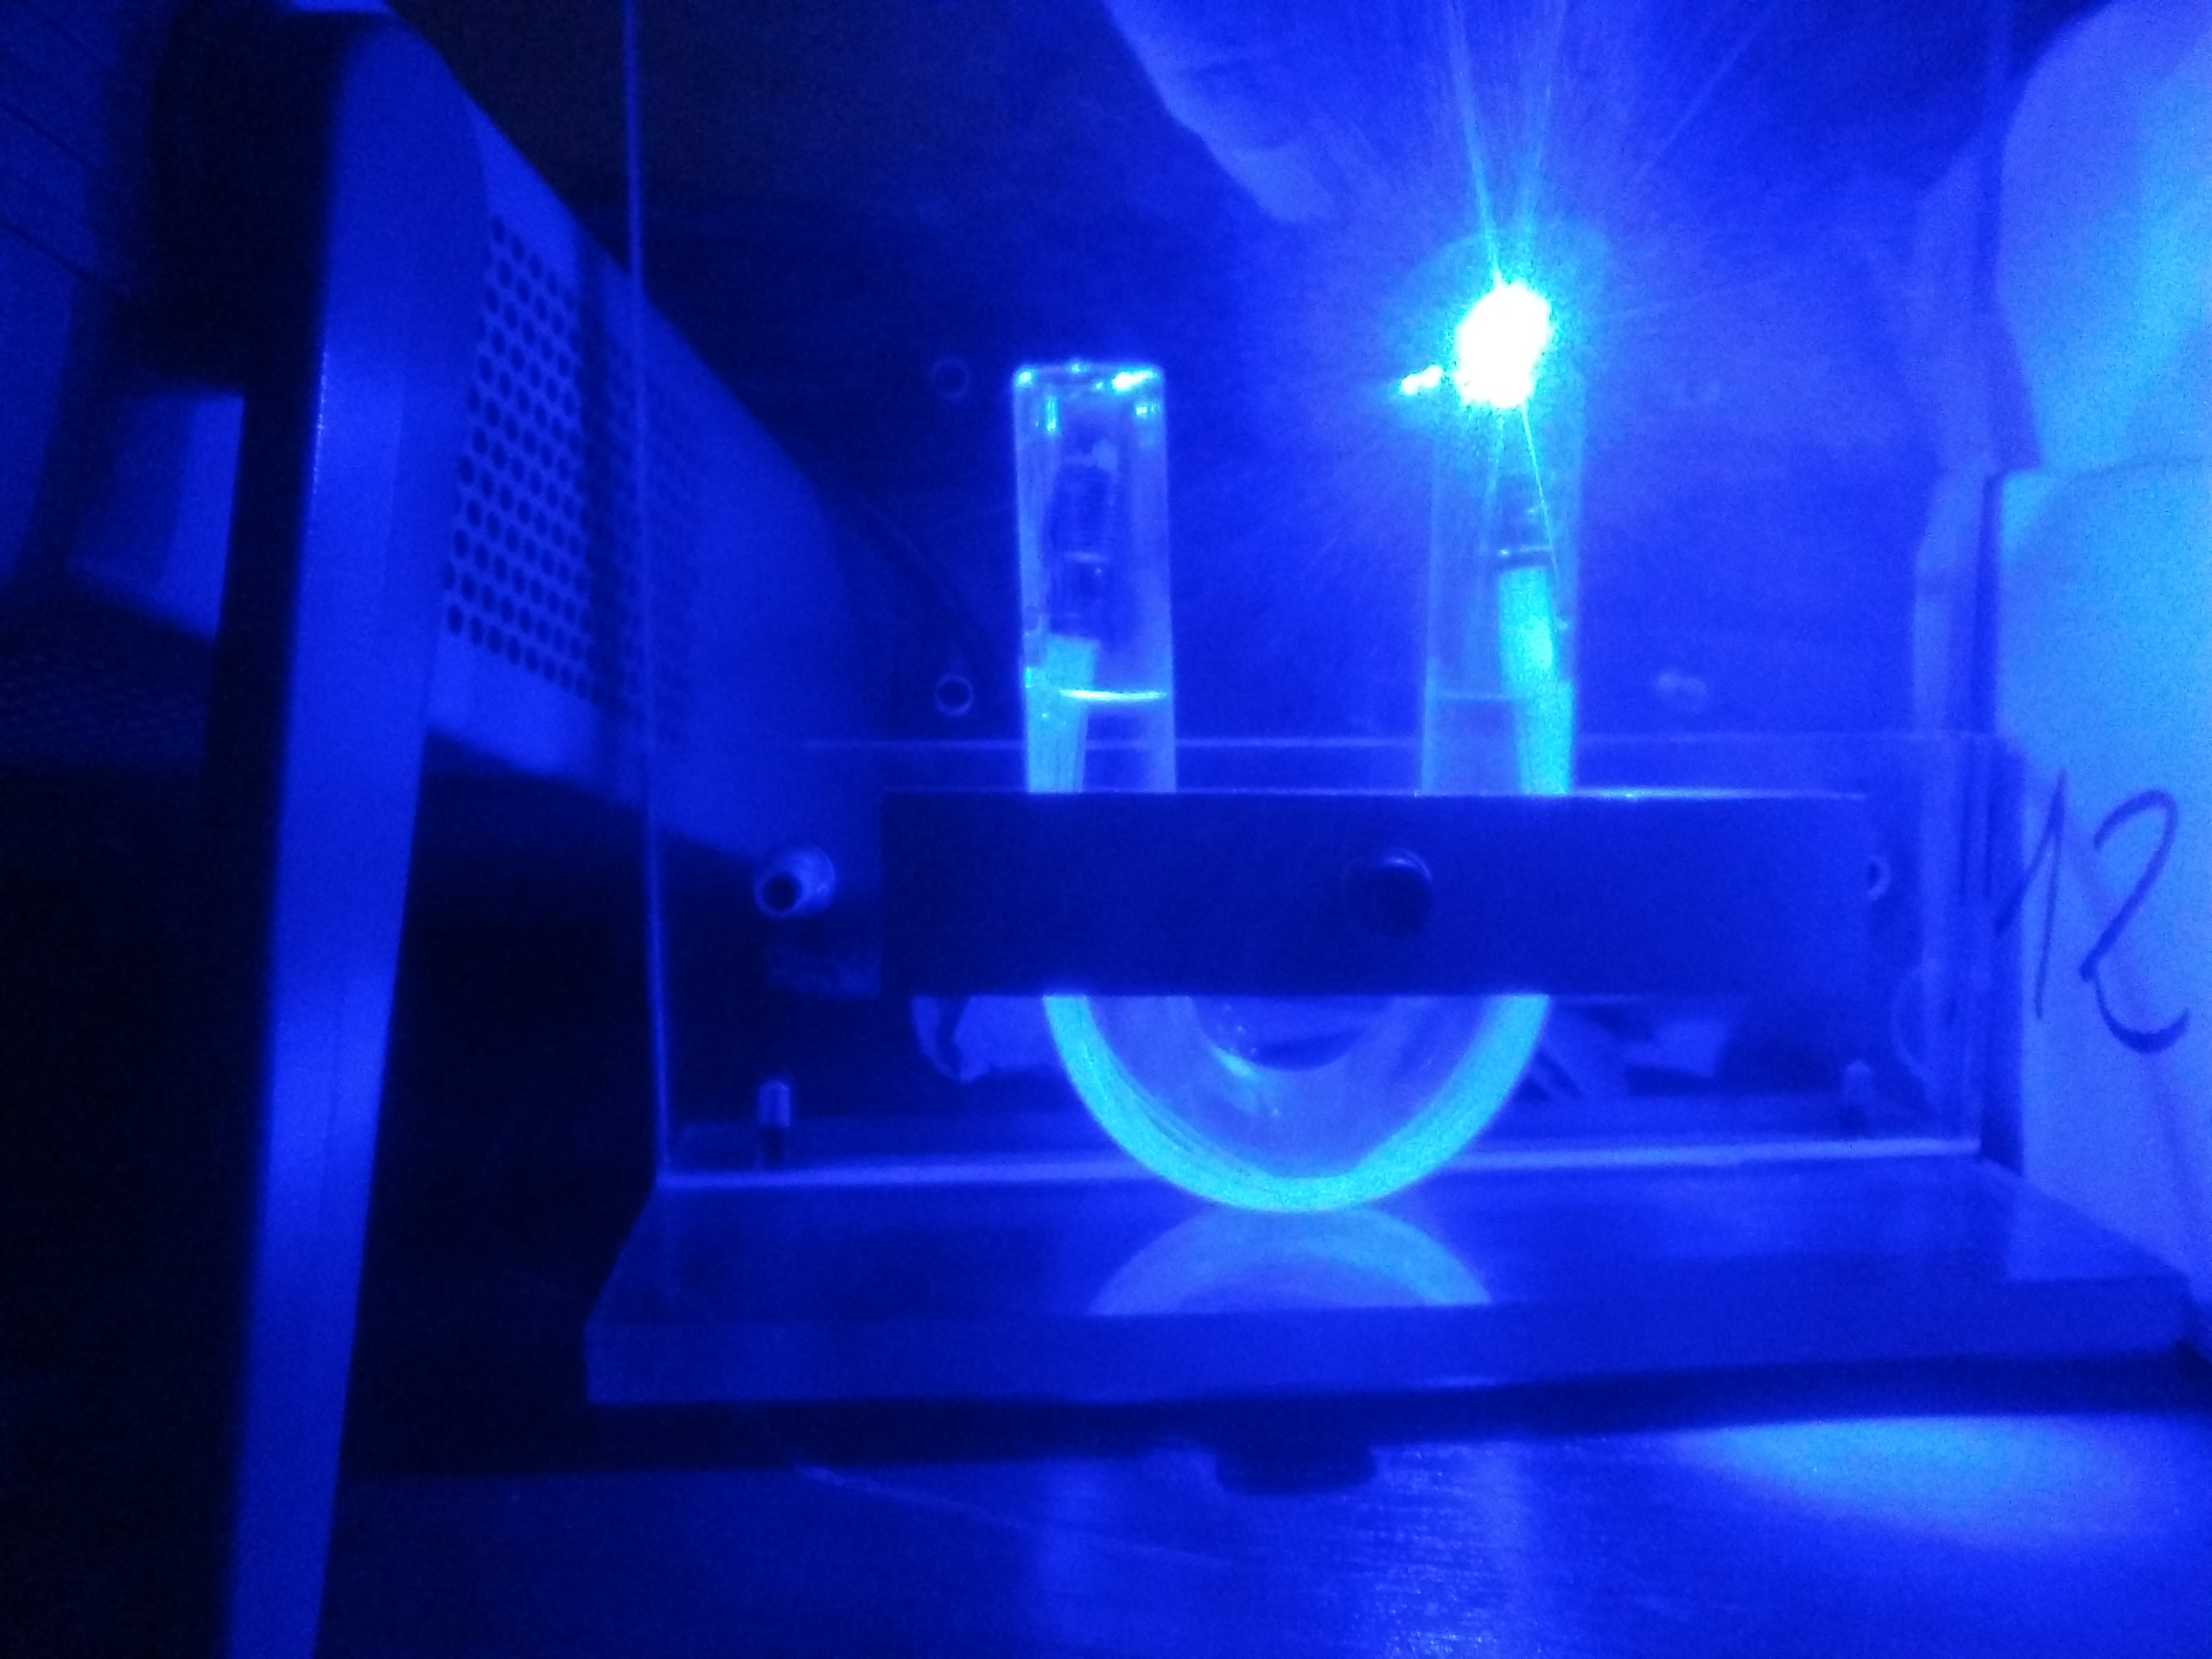
\includegraphics[width=\textwidth]{5Prototypes/52PreliminarPrototypes/521TritiumIFIC0/Lost_Photons.jpg}  
    \caption{\label{subfig:TestLostPhotons}}
    \end{subfigure}
 \caption{a) Fibre bundle in a PMMA vessel. b) Illumination test of the bundle to visualize the light loss due to fibre curvature.}
 \label{fig:TestLostPhotons}
\end{figure}

Data with TRITIUM-IFIC-0 were taken with a single PMT. The energy spectra measured for both the signal and background prototypes are shown in Figure \ref{subfig:SignalBackgroundEnergySpectraTritiumIFIC0}. The difference between signal and background, shown in Figure \ref{subfig:TritiumEnergySpectraTritiumIFIC0}, corresponds to the energy spectrum of tritium. The counting rates obtained for the three spectra are given in Table \ref{tab:CountsPerSecondTRITIUMIFIC0}.
\begin{figure}
\centering
    \begin{subfigure}[b]{1\textwidth}
    \centering
    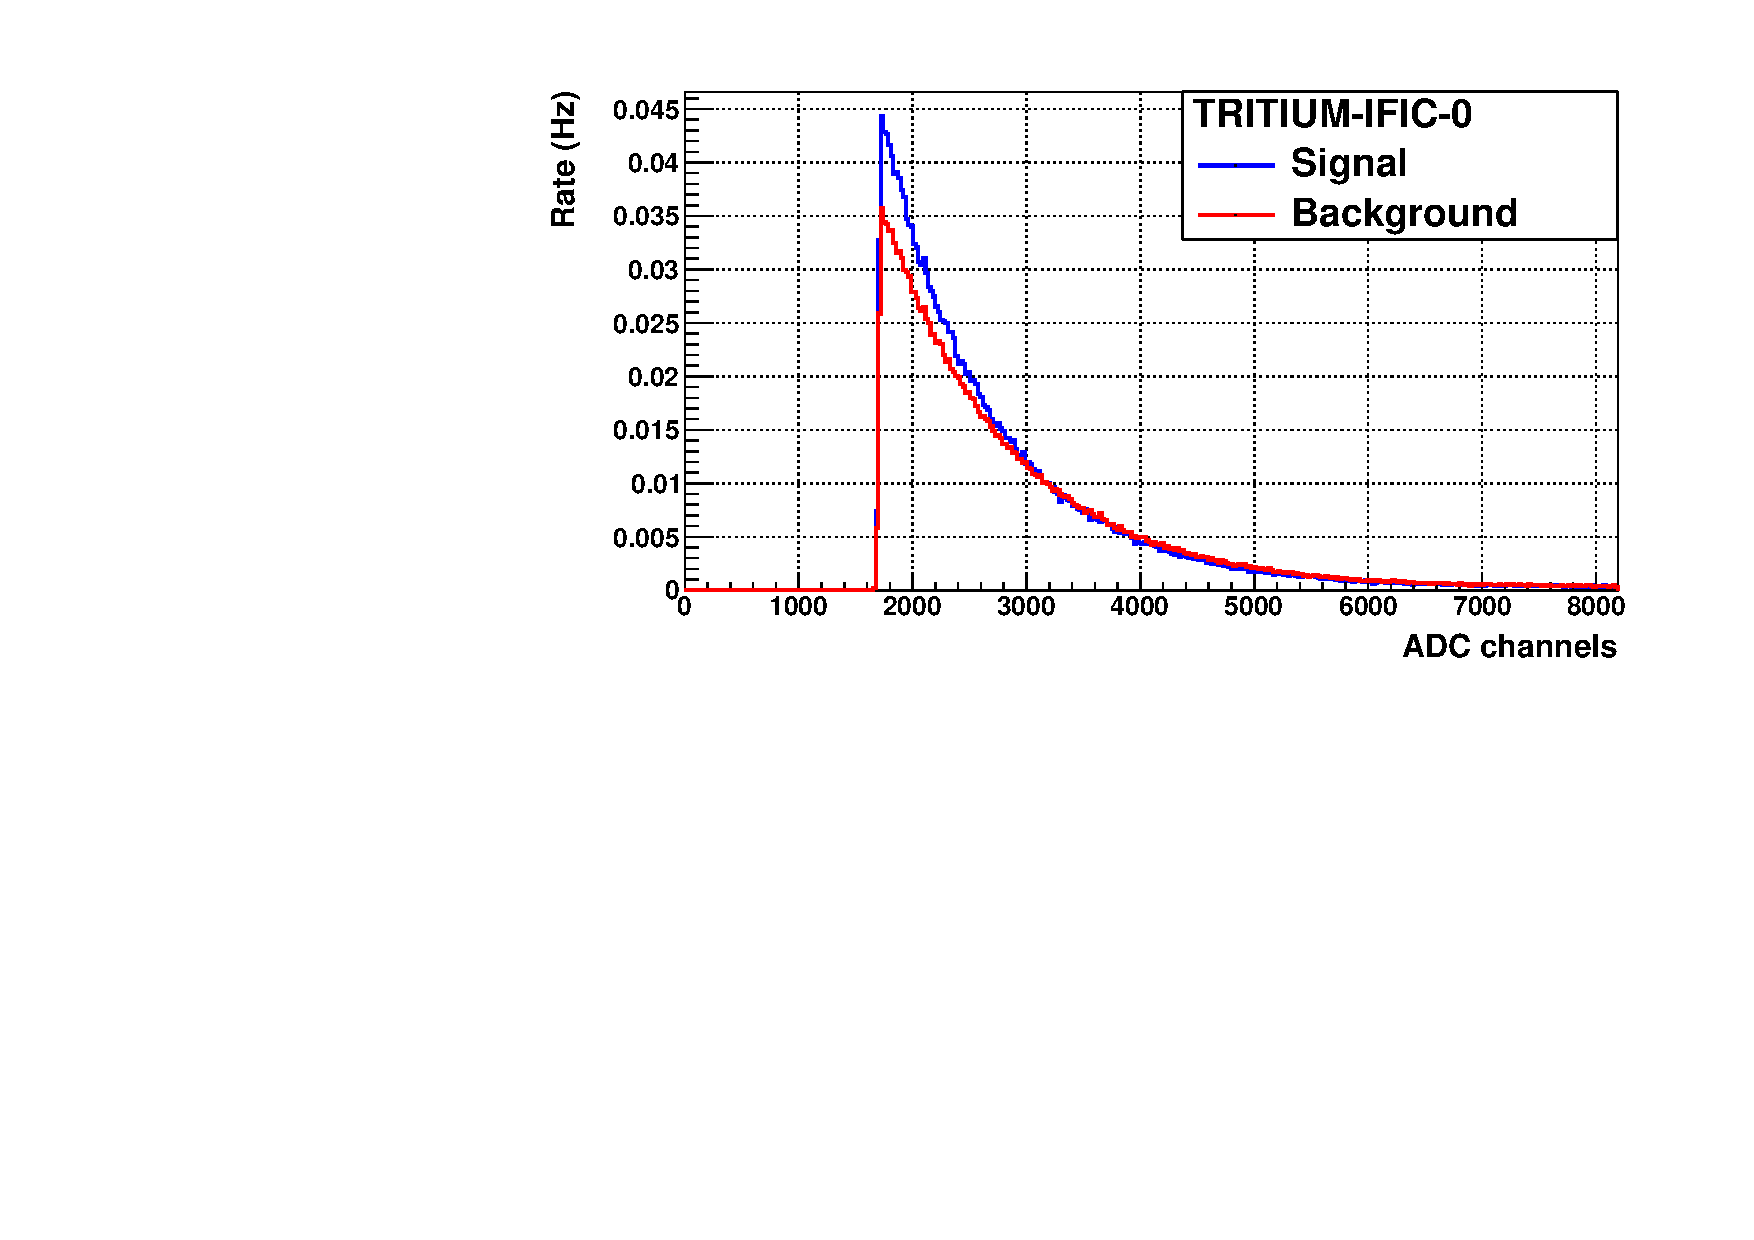
\includegraphics[width=\textwidth]{5Prototypes/52PreliminarPrototypes/521TritiumIFIC0/TritiumIFIC0Signals.pdf}  
    \caption{.\label{subfig:SignalBackgroundEnergySpectraTritiumIFIC0}}
    \end{subfigure}
    \hfill
    \begin{subfigure}[b]{1\textwidth}
    \centering
    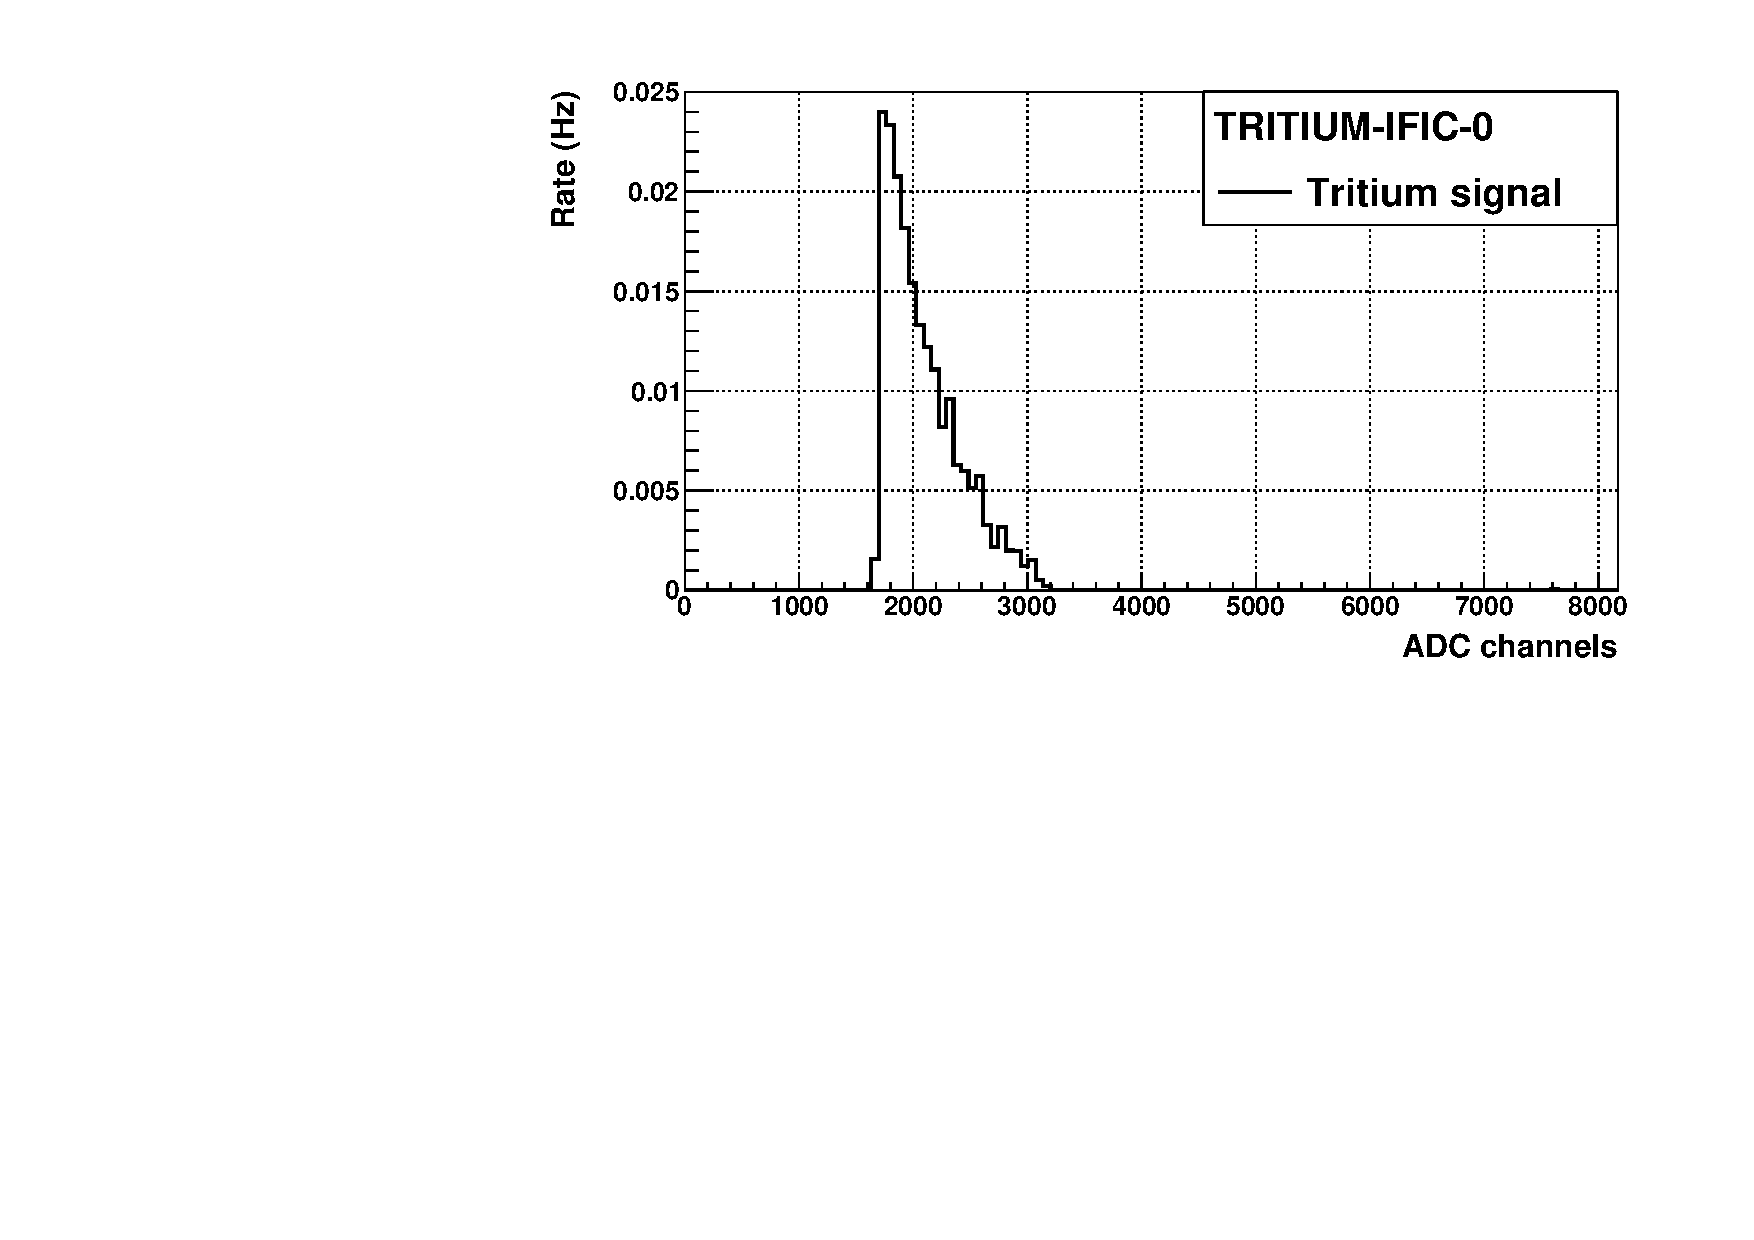
\includegraphics[width=\textwidth]{5Prototypes/52PreliminarPrototypes/521TritiumIFIC0/TritiumIFIC0ClearRebin.pdf}  
    \caption{\label{subfig:TritiumEnergySpectraTritiumIFIC0}}
    \end{subfigure}
 \caption{Energy spectra measured by TRITIUM-IFIC-0. a) Signal and background energy spectra. b) Tritium energy spectrum.}
 \label{fig:EnergySpectraTRITIUMIFIC0}
\end{figure}
\begin{table}[htbp]
\centering{}%
\begin{tabular}{cc}
\toprule 
Spectrum & Rate (Hz) \tabularnewline
\midrule
\midrule 
Signal & $2.27 \pm 0.06$ \tabularnewline
Background & $2.06 \pm 0.06$ \tabularnewline  
Tritium & $0.21 \pm 0.09$ \tabularnewline
\bottomrule
\end{tabular}
\caption{Rates obtained by TRITIUM-IFIC-0.}
\label{tab:CountsPerSecondTRITIUMIFIC0}
\end{table}
The tritium detection efficiency obtained by TRITIUM-IFIC-0, calculated as the ratio of the tritium counting rate to the specific activity of the tritium liquid source, is $$\eta=(2.1 \pm 0.9)\cdot{} 10^{-3}~\liter\:\kilo\becquerel^{-1}\second^{-1}$$
As reported in section \ref{sec:StateOfTheArt}, the tritium detection efficiency scales with the active area of the scintillator used. Therefore, to compare the efficiency with other detectors in the literature and with other prototypes developed in the TRITIUM project, the specific efficiency $S$, calculated by normalizing the detection efficiency to the scintillator area, is
$$S = (9.6 \pm 3.9)\cdot{} 10^{-6}~\liter\:\kilo\becquerel^{-1}\second^{-1}\cm^{-2}$$
As can be seen in Table \ref{tab:PlasticScinTritium}, the specific efficiency is somewhat larger than that obtained by Muramatsu \cite{Muramatsu}, $S=3.13 \cdot{} 10^{-6}~\liter\:\kilo\becquerel^{-1}\second^{-1}\cm^{-2}$, and similar to that obtained by Moghissi \cite{Moghissi}, $S=10.6 \cdot{} 10^{-6}~\liter\:\kilo\becquerel^{-1}\second^{-1}\cm^{-2}$. These efficiencies are too low to achieve the objective of measuring activities of the order of $100~\becquerel/\liter$. 

%In addition, some improvements was applied to next prototype, Tritium-IFIC-1. On the one hand, the special cleaning protocol, previously explained in section \ref{subsubsec:CleaningProcess}, was applied on the fibres. It was used to improve the interfaces between fibre and tritiated water, creating a better wetting property of the fibre, which will result in more tritium events detected and a greater photon collection efficiency.

%On the other hand, as we have seen in our previous characterization study of the fibres, shown in section \ref{subsubsec:CharacterizationFibers}, the photon collection efficiency of the fibres used is poor, so a large number of photons will be lost in each tritium event.

%It is an innerent characteristic of the fibre which we cannot change but, to reduce its effect, we will use a Teflon vessel for our next prototypes.

%Teflon is an interesting material for its optical properties, specifically its reflection factor, which is very close to $100\%$ at the working wavelength. It means that practically all the photons that reach the walls of the vessel will be reflected back to the fibre.

%On the other hand, the fibres were inspected under the electronic microscope of the SCSIE \cite{ElectronicMicroscopeSCSIE}, with which we can see details of the order of tens of nanometers.

%The result is shown in Figure \ref{}, where you can see many irregularities of the order of $X~\nm$. These irregularities will cause photons to escape from the fibre. It is a characteristic of the fibres that we cannot change but, to reduce its effect, we will use a Teflon vessel for our next prototypes.

%FOTOOOO

%Teflon is an interesting material for its optical properties, specifically its reflection factor. Its reflection factor is very close to $100\%$ at the working wavelength, which means that practically all the photons that reach walls of the vessel will be reflected back to the fibre.